\documentclass[main.tex]{subfiles}
\begin{document}

\section{Grammatical Relations}
 

The simplest classification approach used in this study considered the relative frequency of different grammatical relations. For this approach, the governor and the dependent of the dependencies were ignored, with only the relation itself being used. 

Each data set instance contained attributes corresponding to dependency relations. The Stanford parser system in its default configuration does not generate the \textit{punct} or punctuation dependency which connects punctuation symbols to a key element in the associated clause. Since English punctuation is broadly similar to Spanish punctuation, aside from some stark differences such as Spanish's inverted question and exclamation marks, which should be apparent to even the beginning learner, it did not seem to useful to activate this dependency. Additionally, the \textit{abbrev} or abbreviation dependency was removed. This dependency marks the definition of an abbreviation, as in the example given by \citet{typed-deps-manual}, ``Australian Broadcasting Corporation (ABC)'', where the dependency would be $abbrev(\text{Corporation},\text{ABC})$. This dependency has little to do with grammar, and thus was ignored for the purposes of this study. Having excluded these two dependencies, each data set instance contained 58 numerical attributes, one for each relation used.

      For each attribute $A_r$ corresponding to the relation $r$, the corresponding value was the floating point number $n_r/n_t$, where $n_r$ and $n_t$ were the number of occurrences of the relation $r$ and the total number of relations in the text, respectively. A C4.5 decision tree classifier trained on these instances produces the decision tree shown in Figure~\ref{fig:c4.5-dep-tree}, employing 15 different relations. The full names for these relations are shown in Table~\ref{table:reln-abbr}. At each terminal node of the tree there is an integer or pair of integers in parentheses. These values indicate the number of the training cases that were categorized (correctly or not) at that node and the number of cases incorrectly categorized, this latter value only being shown when greater than zero. For any given test node, one can identify one branch as the predominately \textit{en} branch and the other as the \textit{es} branch. For test nodes where one or both branches lead to terminal nodes, this is trivial, as the terminal nodes themselves label the branches. For any other test node, the branches can be identified by summing up the number of test cases at the terminal nodes of that branch. For instance, the root test node, which considers the relation \textit{nn}, divides the training set of 642 cases into a subset of 337 cases, associated with the left branch, and another subset of 305 cases, associated with the right branch. Looking at the left branch, it can be seen that of these 336 cases, 301 of them are nonnative, i.e. of the class \textit{es}, and only 36 are native. This indicates that this is a predominately nonnative branch. Conversely, the right hand branch consists of 205 native cases and only 20 nonnative cases, making it the native branch. This allows one to say, for instance, that fewer occurrences of the \textit{nn} relation are associated with nonnative samples. The following subsections explore the linguistic reasons why these relations should be so useful in making such categorizations.

\begin{figure}
\centering
\caption{C4.5 decision tree employing relative frequency of dependency relations. Relative frequencies are shown as percentages. Values in parentheses are the number of training case classified at that point and, following the slash when present, the number of those cases which were incorrectly classified.}
\label{fig:c4.5-dep-tree}
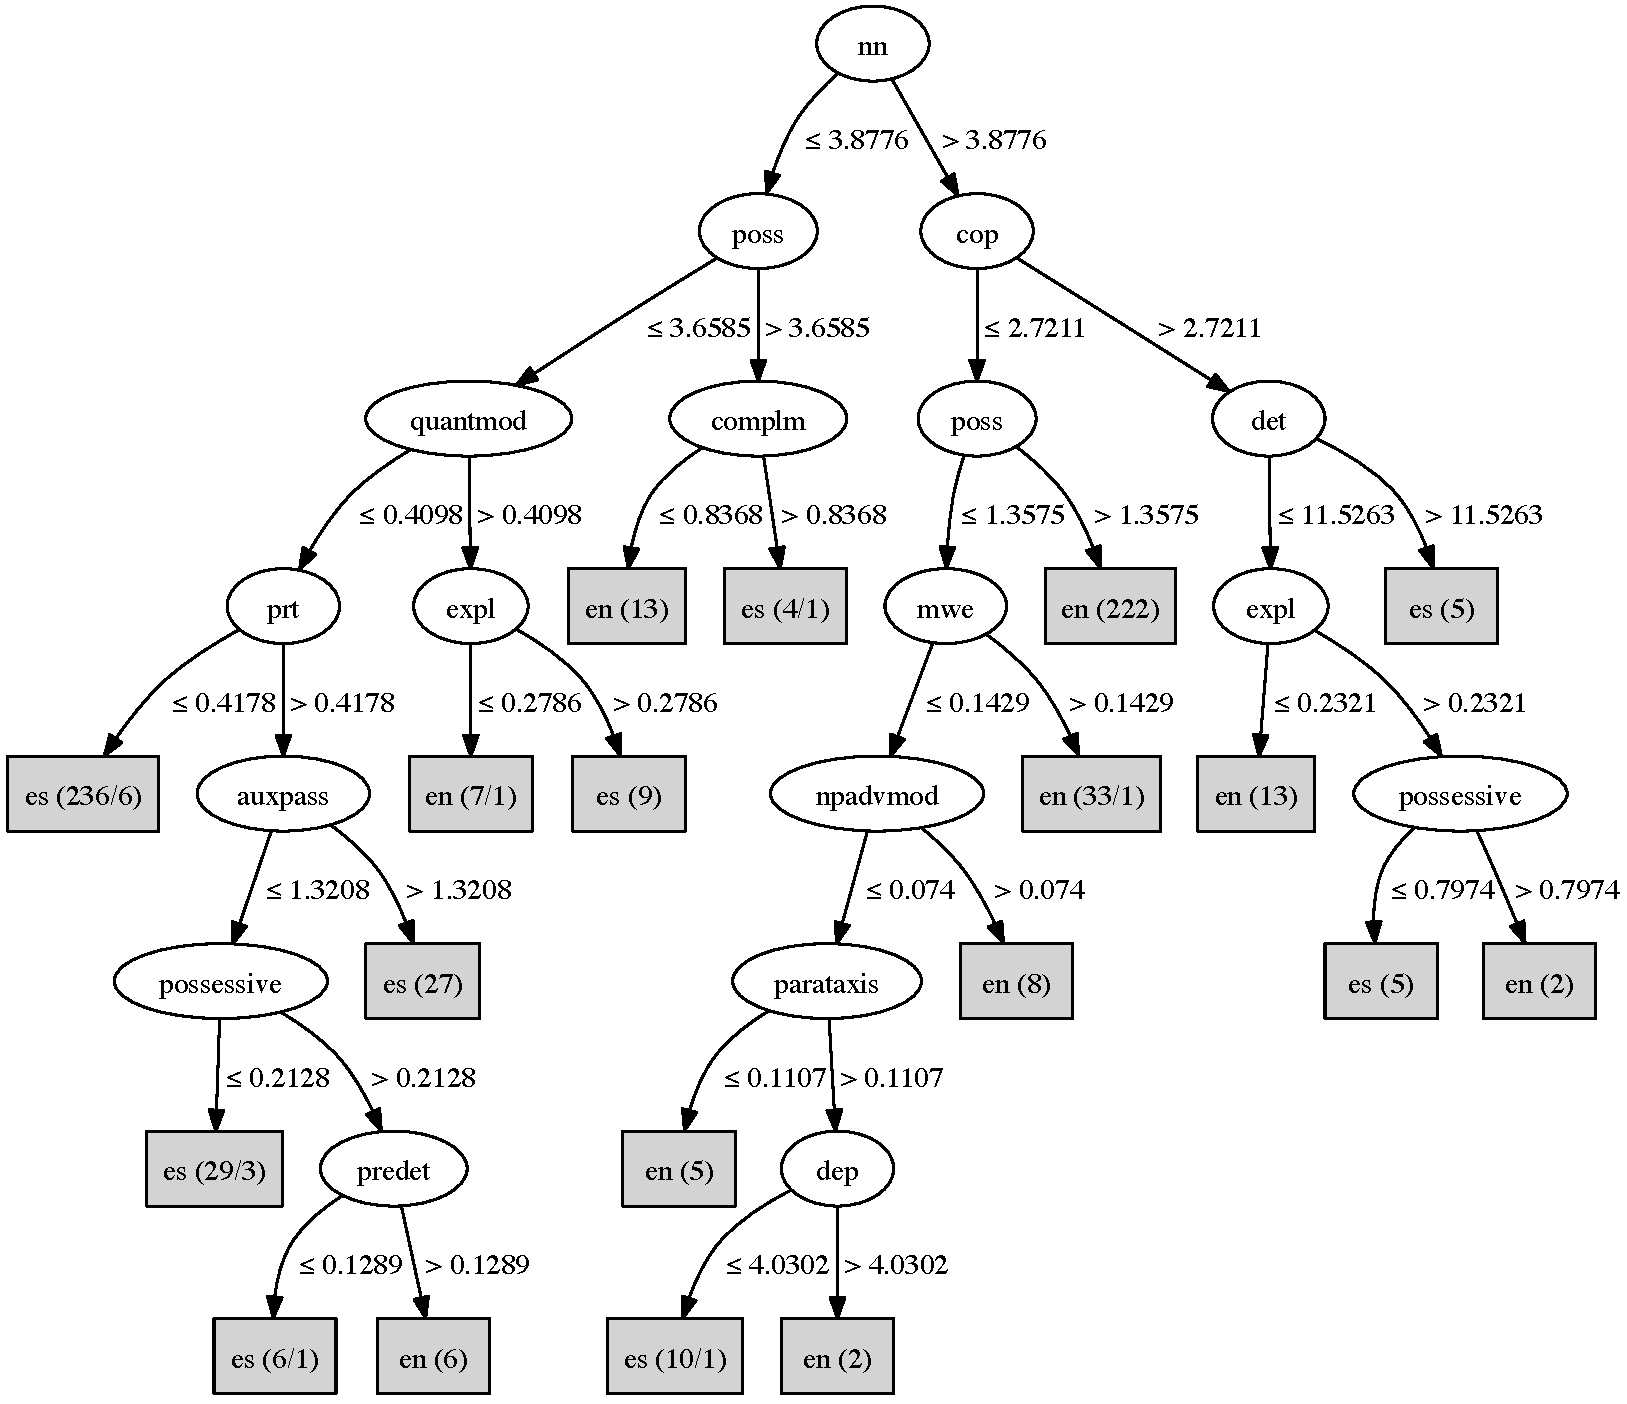
\includegraphics[width=6in]{c45-dep-graph.pdf}
\end{figure}



\begin{table}
\small
\centering
\caption{Relation abbreviations}
\begin{tabular}{ l  l }
    \toprule
$auxpass$ & passive auxiliary \\
$complm$ & complementizer \\
$cop$ & copula \\
$det$ & determiner \\
$expl$ & expletive\\
$mwe$ & multi-word expression \\
$nn$ & noun compound modifier \\
$npadvmod$ & noun phrase as adverbial modifier \\
$parataxis$ & parataxis \\
$poss$ & possession modifier \\
$possessive$ & possessive modifier \\
$predet$ & preconjunct \\
$prt$ & phrasal verb particle \\
$quantmod$ & quantifier phrase modifier \\
$rel$ & relative \\
\bottomrule
\end{tabular}
\label{table:reln-abbr}
\end{table}


\subsection{Passive Auxiliary}

The passive auxiliary dependency \textit{auxpass} marks an auxiliary verb which carries the passive information of the clause. In general a parsed sample of text will contain one such dependency for every passive clause and so a high relative frequency of this relation indicates heavy usage of the passive voice. Example~\ref{ex:auxpass-dep} illustrates this dependency.

\begin{figure}
\caption{The dependencies $auxpass(\text{killed},\text{been})$ and $auxpass(\text{killed},\text{was/got})$. Taken from \citet{typed-deps-manual}.}

\centering
\begin{tabular}{ l l }
a. & \xytext{
\xybarnode{Kennedy} &
\xybarnode{has} &
\xybarnode{been} &
\xybarnode{killed}
\xybarconnect(U,U){-1}"_{\small auxpass}"
}\\
b. & \xytext{
\xybarnode{Kennedy} &
\xybarnode{was/got} &
\xybarnode{killed}
\xybarconnect(U,U){-1}"_{\small auxpass}"
}
\end{tabular}
\label{ex:auxpass-dep}
\end{figure}


\subsection{Complementizer}

A complementizer is a word that signals the beginning of a clausal complement. The Stanford Parser recognizes the complementizers \textit{that} and \textit{whether} as shown in Example~\ref{ex:complm3}. The governor of a complementizer dependency is the root of the clause, which is generally a verb or, in the cause of copular clauses, the subject complement. The dependent is the complementizer itself.


\begin{figure}
\caption{The dependencies $complm(\text{place},\text{whether})$, $complm(\text{go},\text{whether})$ $complm(\text{predicts},\text{that})$, and $complm(\text{rise},\text{that})$. Nonnative samples from WRICLE (\textit{a} and \textit{c}) and SULEC (\textit{b}).}

\centering
\begin{tabular}{ l l }
a. &
\xytext{
\xybarnode{\ldots} &
\xybarnode{I} &
\xybarnode{will} &
\xybarnode{consider} &
\xybarnode{\ldots} &
\xybarnode{whether} &
\xybarnode{the} &
\xybarnode{world} &
\xybarnode{is} &
\xybarnode{a} &
\xybarnode{safe} &
\xybarnode{place}
\xybarconnect(U,U){-6}"_{\small complm}"
}\\

b. &
\xytext{
\xybarnode{At} &
\xybarnode{least} &
\xybarnode{you} &
\xybarnode{choose} &
\xybarnode{whether} &
\xybarnode{to} &
\xybarnode{go}
\xybarconnect(U,U){-2}"_{\small complm}" &
\xybarnode{to} &
\xybarnode{a} &
\xybarnode{pub} &
\xybarnode{or} &
\xybarnode{not.}
}\\

c. &
\xytext{
\xybarnode{They} &
\xybarnode{state} &
\xybarnode{that} &
\xybarnode{climate} &
\xybarnode{generally} &
\xybarnode{predicts}
\xybarconnect(U,U){-3}"_{\small complm}"&
\xybarnode{that} &
\xybarnode{temperatures} &
\xybarnode{should} &
\xybarnode{rise}
\xybarconnect(U,U){-3}"_{\small complm}"&
\ldots
}
\end{tabular}
\label{ex:complm3}
\end{figure}


\citet{whitley:1986} points out that while English tends to allow complementizers introducing clausal complements in the object position to be deleted, Spanish is much more restrictive in this regard (see examples~\ref{ex:complm1} and~\ref{ex:complm2}). \citep[p.278]{whitley:1986}.

\begin{figure}
\eenumsentence{
\label{ex:complm1}
\item I say that he'll do it.
\item I say he'll do it.
}

\eenumsentence{
\label{ex:complm2}
\item Digo que lo hará.
\item *Digo lo hará.
}
\end{figure}

\subsection{Copula}

The copula or $cop$ dependency marks the copular verb. This dependency takes as its governor the complement of the copular clause and the verb itself as the dependent. 

\subsection{Determiner}

The determiner or $det$ dependency connects a determiner to the NP it modifies with the determiner being the dependent and the head of the NP the governor.

\subsection{Expletive}

An existential \textit{there} and the copular verb associated with it are connected with the expletive or $expl$ relation.

\subsection{Multi-Word Expression}

The Stanford typed dependency manual \citep{typed-deps-manual} defines multi-word expressions as being two or more words that are used together as a single unit such that the relationship between them is difficult to define. In the version of the Stanford parser used here, only the following expression are considered multi-word expressions: \textit{rather than, as well as, instead of, such as, because of, in addition to, all but, due to}.

\subsection{Noun Compound Modifier}

Noun-noun compounds (NNCs) are marked with the relation \textit{nn}. The governor of this dependency is the rightmost noun in the compound and the dependent will be one of the nouns to the left. Note that since all dependencies only deal with pairs of words, a compound consisting of more than two nouns would be indicated by multiple dependencies, all sharing a common governor. Example~\ref{fig:nn-deps} demonstrates this dependency. 

\begin{figure}[htbp]
\caption{The dependency $nn(\text{concentration}, \text{oxygen})$. Native sample taken from MICUSP.}
\centering
\xytext{
\xybarnode{\ldots} &
\xybarnode{oil}
%\xybarconnect(D,D){1}"_{\small possessive}"&
\xybarnode{'s} &
\xybarnode{effects} &
%\xybarconnect(U,U){-2}"_{\small poss}"&
\xybarnode{on} &
\xybarnode{dissolved} &
\xybarnode{oxygen} &
\xybarnode{concentration} 
\xybarconnect(U,U){-1}"_{\small nn}"&
\xybarnode{led} &
\xybarnode{me} &
\xybarnode{to} &
\xybarnode{\ldots}
}
\label{fig:nn-deps}
\end{figure}

\subsection{Noun Phrase as Adverbial Modifier}



\subsection{Parataxis}
\subsection{Possession and Possessive Modifiers}

Inflected genitive constructions are marked by two dependencies: \textit{poss}, which ties the head of a NP (the governor) to a genitive inflectional suffix (\textit{'s}~or~\textit{'}), indicating that the governor is the possessed element; and \textit{possessive}, which connects a noun to its own genitive inflectional suffix. These two dependencies are illustrated in Figure~\ref{fig:poss-deps}. The $poss$ dependency can also have as its dependent a possessive determiner such as \textit{its} or \textit{their}. In this type of construction, the $possession$ dependency is not used. 

\begin{figure}[htbp]
\caption{The dependencies $poss(\text{effects}, \text{oil})$ and $possessive(text{oil}, \text{'s})$. Native sample taken from MICUSP.}
\centering
\xytext{
\xybarnode{\ldots} &
\xybarnode{oil} \xybarconnect(D,D){1}"_{\small possessive}"&
\xybarnode{'s} &
\xybarnode{effects} 
\xybarconnect(U,U){-2}"_{\small poss}"&
\xybarnode{on} &
\xybarnode{dissolved} &
\xybarnode{oxygen} &
\xybarnode{concentration} &
\xybarnode{led} &
\xybarnode{me} &
\xybarnode{to} &
\xybarnode{\ldots}
}
\label{fig:poss-deps}
\end{figure}

\subsection{Preconjunct}

The preconjunct ($preconj$) dependency connects the head of a phrase employing a conjunction to a word that emphasizes or brackets that conjunction, such as \textit{either}, \textit{neither}, or \textit{both}. Figure~\ref{fig:preconj-dep} demonstrates this dependency.

\begin{figure}[h]
\caption{The dependencies $preconj(\text{boys},\text{both})$ and $preconj(\text{emotionally},\text{neither})$. (a) taken from \citet{typed-deps-manual} and (b) from WRICLE (nonnative).}
\centering
\begin{tabular}{ l l }
a. &
\xytext{
\xybarnode{Both} &
\xybarnode{the} &
\xybarnode{boys} 
\xybarconnect(U,U){-2}"_{\small preconj}"&
\xybarnode{and} &
\xybarnode{the} &
\xybarnode{girls} &
\xybarnode{are} &
\xybarnode{here.} &
}
\\

b. &
\xytext{
\xybarnode{\ldots are} &
\xybarnode{neither} &
\xybarnode{emotionally} 
\xybarconnect(U,U){-1}"_{\small preconj}" &
\xybarnode{nor} &
\xybarnode{economically} &
\xybarnode{prepared \ldots}
}

\label{fig:preconj-dep}
\end{tabular}
\end{figure}


\subsection{Phrasal Verb Particle}

The phrasal verb particle relation ($prt$) ties the head word of a phrasal verb to its particle as shown in Example~\ref{ex:prt-en1}. The decision tree in Figure~\ref{fig:c4.5-dep-tree} contains this relation once. Relative frequencies of less than or equal to 0.4178\% lead to the categorization of a text as nonnative, whereas larger values lead to a subtree. It can be seen that a very high percentage, 36.8\%, of the training cases terminate at the left, or nonnative, branch of this test node, suggesting that this relation contributes a great deal of useful information to the categorization process.

\begin{figure}[h]
\caption{The dependency $prt(\text{free},\text{up})$. Native sample from MICUSP.}
\centering
\xytext{
\xybarnode{\ldots the} &
\xybarnode{reduction} &
\xybarnode{of} &
\xybarnode{superfluous} &
\xybarnode{proteins} &
\xybarnode{will} &
\xybarnode{free}
\xybarconnect(U,U){1}"^{\small prt}"
&
\xybarnode{up} &
\xybarnode{resources \ldots}
}
\label{ex:prt-en1}
\end{figure}

Phrasal verbs are multiword verbs consisting of a core word, which can generally stand alone as a distinct verb in other circumstances, and a preposition-like particle appearing after, though in many cases not immediately after, the primary word \citep{celce-murcia:1999}. These verbs appear to be rare in world languages, with few non-Germanic languages containing such constructions \citep{celce-murcia:1999}. \citet{liao:2004} conduct a review of the literature on phrasal verb avoidance in English language learners, starting with \citep{dagut:1985}, a study which concluded that L1-Hebrew learners of English do avoid these verbs. They further asserted that the reason for this was syntactic differences between Hebrew and English, though others have questioned their bases for this assertion \citep{liao:2004}. The review continues with \citep{hulstijn:1989}, who investigated the claims of \citeauthor{dagut:1985} by applying their same data gathering techniques to a group of English learners whose first language was Dutch, a language which also uses phrasal verbs. Contrary to their expectations, they found that the Dutch speakers did not avoid phrase verbs in English, suggesting that L1-interference is, at least in part, the source of phrasal verb avoidance. Finally, the review cites the study of \citet{laufer:1993}, which performed a very similar study as \citeauthor{hulstijn:1989}, but with native Swedish speakers, and made much the same conclusions.

In their own study, \citeauthor{liao:2004} investigate L1-Chinese learners of English, and cautiously concluded that the syntactic features of Chinese lead to the avoidance of phrasal verbs in the English of those learners. A later study, \citet{gonzalez:2010}, uses the Spanish and Swedish subcorpora of ICLE along with the British National Corpus (BNC), a corpus of native written English, to perform a quantitative study of phrasal verb usage. They found that the L1-Swedish learners used phrasal verbs 69\% as often as the native speakers and the L1-Spanish learners used phrasal verbs 45\% as often. These numbers would seem to indicate that the syntax of the learner's L1 is an important, but not the only, contributing factor to phrasal verb avoidance.

Regardless of the reasons behind L1-Spanish learners avoidance of phrasal verbs, \citet{gonzalez:2010} demonstrates that it is a reality of learner English. Considering this, it is not surprising that the C4.5 algorithm uses the $prt$ relation with such success in the categorization process.


\subsection{Quantifier Phrase Modifiers}
\subsection{Relative}


\biblio
\end{document}
